\documentclass[10pt]{beamer}

\usetheme[progressbar=frametitle]{metropolis}
\usepackage{appendixnumberbeamer}

\usepackage{booktabs}
\usepackage[scale=2]{ccicons}

\usepackage{pgfplots}
\usepgfplotslibrary{dateplot}

\usepackage[utf8]{inputenc}

\usepackage{xspace}
\newcommand{\themename}{\textbf{\textsc{metropolis}}\xspace}

\title{Better Online Deterministic Packet Routing on Grids}
\subtitle{Számítógép-hálózatok és osztott rendszerek}
\date{\today}
\author{Kádár Tamás Csaba, Kedves Nándor}

\begin{document}

\maketitle

\begin{frame}{Tartalomjegyzék}
  \setbeamertemplate{section in toc}[sections numbered]
  \tableofcontents[hideallsubsections]
\end{frame}

\section{Bevezetés}

\begin{frame}[fragile]{Modell}

  Hálózatunkat a következő modellel írjuk le, melyet \cite{even2015better} cikk alapján építjük fel:
  \begin{itemize}
  	\item $ G = \left( V, E \right) $ irányított gráf
  	\item $ B $ buffer méret, $ c $ élek kapacitása, ahol $ B, c > 0 $
  \end{itemize}

  A hálózat topológiája irányított egyenes, amely $ n $ vertexből áll $ V = \left\lbrace v_0, v_1,\dots,v_{n-1} \right\rbrace, E = \left\lbrace \left( v_{i-1}, v_i \right) | \ 0 < i < n \right\rbrace $

  \begin{figure}[c]
  	\centering 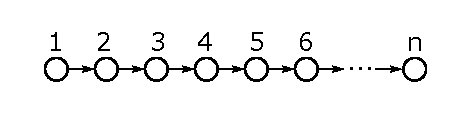
\includegraphics[width=1\columnwidth]{Image/linear_network}
  	\caption{\label{fig:linear_network}Lineáris hálózatmodell}
  \end{figure}

\end{frame}

\begin{frame}{Kérés (Request)}
  A kérést egy számhármassal adhatjuk meg, $ r = \left(a_i, b_i, t_i \right)  $
  \begin{itemize}
  	\item $ a_i $ a forrás csomópont
  	\item $ b_i $ a cél csomópont
  	\item $ t_i $ az időpont amikor a kérés érkezik
  \end{itemize}
 , ahol $ a_i, b_i \in V, t_i \in \mathbb{N} $\newline
 Minden time stepben, a routing algoritmus:
 \begin{itemize}
 	\item törli a célba érkezett csomagokat
 	\item minden más csomagra, beleértve az éppen beérkezőket is eldönti, hogy:
	 \begin{itemize}
	 	\item törli
	 	\item tárolja az aktuális csomópont bufferjében
	 	\item továbbküldi a következő vertexnek
	 \end{itemize}
 \end{itemize}
\end{frame}

\section{Modell és probléma}

\begin{frame}{Az egyenes modelltől a rácsmodellig}
	Kiindulunk a már említett modellből és a következő modellt építjük fel:
	\begin{itemize}
		\item 
		$ G^{st} = \left( V^{st}, E^{st} \right) $ irányított aciklikus végtelen gráf, amiben $ c^{st}\left(e \right) $ az élek kapacitása. $ V^{st} := V \times \mathbb{N} $, ahol minden $ v \in V $ vertexnek végtelen számú másolata van a $ G^{st} $-ben, melyet a $ \left( v, t\right) \in V^{st} $ azonosít. $ E^{st} := E_0 \cup E_1 $, ahol az $ E_0 $ tartalmazza a csomópontok közötti éleket, melyek $ c $ kapacitással rendelkeznek és a $ E_1 $ a ugyanazon csomópont time steppek közötti élét tartalmazza, mely kapacitása $ B $
 		\item  a kérés a következőképpen alakul $ r_i^{st} = \left( \left( a_i, t_i\right) , row(b_i)\right) $, ahol a $ row(b_i) $, a cél csomópont sorát jelöli
	\end{itemize}
\end{frame}

\begin{frame}{Az egyenes modelltől a rácsmodellig}
	\begin{figure}
		\centering 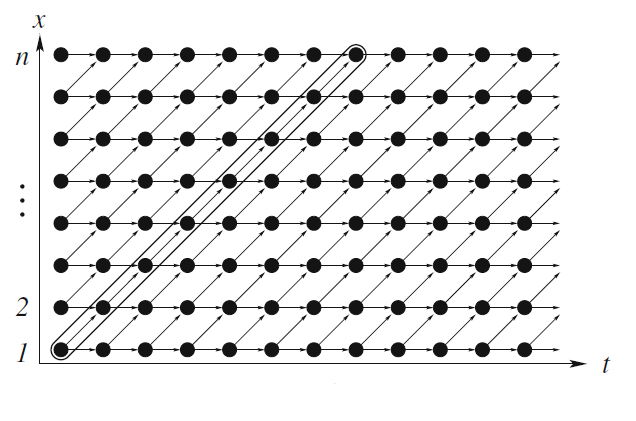
\includegraphics[width=0.8\columnwidth]{Image/grid_network}
		\caption{\label{fig:grid_network}Döntött rácsos hálózatmodell \cite{even2016}}
	\end{figure}
\end{frame}

\begin{frame}{Az egyenes modelltől a rácsmodellig}
	\begin{figure}
		\centering 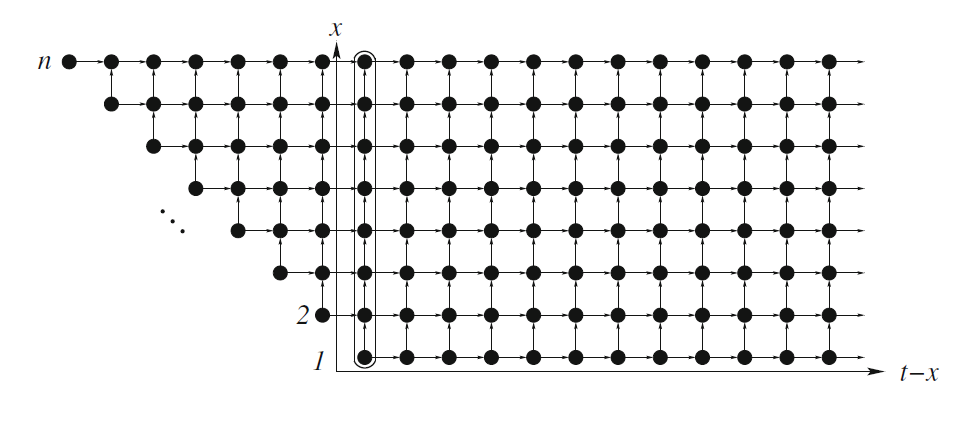
\includegraphics[width=1\columnwidth]{Image/grid_network_untilted}
		\caption{\label{fig:grid_network_untilted}Nem döntött rácsos hálózatmodell \cite{even2016}}
	\end{figure}
\end{frame}

\begin{frame}{Rács modelltől a vázlat gráfig}
  Felépítjük a \textit{sketch gráfot}, mely egy durvább megközelítése a rács modellnek. Felépítéséhez úgynevezett \textit{tilingokat} használunk.\newline
  Tiling
  \begin{itemize}
  	\item $ \ell_h \times \ell_v $ részrács, ahol $ \ell_h = \left \lceil \frac{6k}{5c'} \right \rceil $ és $ \ell_v = \left \lceil \frac{6k}{5B'} \right \rceil $ ($ c' = \lfloor c/5 \rfloor $, $ B' = \lfloor B/5 \rfloor $ és $ k = log(1 + 3 \cdot p_{max}) $, ahol a $ p_{max} $ később kifejtjük)
  	\item $ \phi_x $ és $ \phi_y $ 2 \textit{offset} paraméter segítségével határozzuk meg (($ \phi_x + i \cdot \ell_h, \phi_y + j \cdot \ell_v $), ahol $ i,j \in \mathbb{N} $)
  \end{itemize}
  A cikk által feldolgozott algoritmus 4 offsetet használ $ (\phi_x, \phi_y) \in \left\lbrace -\ell_h/2.0 \right\rbrace \times \left\lbrace -\ell_v/2.0 \right\rbrace $, ezeket nevezzük $ T_1, \dots, T_4 $-nek.
\end{frame}

\begin{frame}{Az egyenes modelltől a rácsmodellig}
	\begin{figure}
		\centering 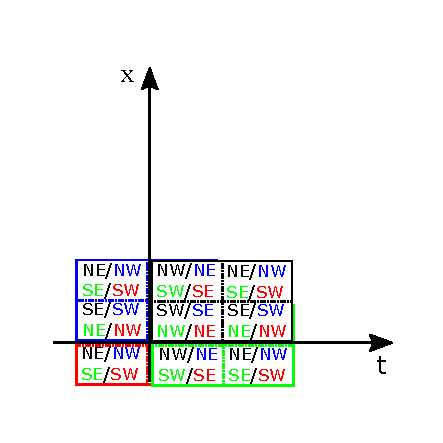
\includegraphics[width=0.8\columnwidth]{Image/sketch_graph}
		\caption{\label{fig:sketch_graph}Sketch gráf}
	\end{figure}
\end{frame}

\begin{frame}{Sketch gráf}
  \begin{alertblock}{Definíció}
	Az $ r_i = (a_i, b_i, t_i) $ kérés $ SW_j $-ben található, ha a forrás vertex $ (a_i, t_i) $ a $ T_j $ csempe délnyugati részéhez tartózik.
  \end{alertblock}
  Egy sketch gráfot indukál a $ T_j $, melyet jelöljük $ S_j := (V(S_j), E(S_j)) $, ahol a $ V(S_j) $ egy csempe halmaz a $ T_j $-ből és nekik van $ (s_1, s_2) \in E(S_j) $, ha $ s_1 \neq s_2 $ és $ E^{st} \cap (s_1 \times s_2) \neq \emptyset $. Minden élhez egy egység kapacitást rendelünk.
\end{frame}

\begin{frame}{Online Packing of Paths}
  \begin{itemize}
  	\item A sketch gráfot használjuk fel az \textit{path packing} probléma megoldásához. Intuitíve a path packing modell hasonlít a packet routing modellhez, kivéve hogy ott nincsenek bufferek és hogy minden link $ e $ különböző kapacitással rendelkezik, melyet a következőképpen jelölünk $ c(e) $.
	\item Formálisan egy kérés a következő alakba írható fel a $ G $ gráfban $ (a_i, D_i) $, ahol $ a_i \in V $ a forrás vertex és a $ D_i \subseteq V $ célrészhalmaz.
    \item Legyen $ P(r_i) $, mely jelölje azon pathek halmazát, melyek kiszolgálják a $ r_i $ kérést. Minden $ p \in P(r_i) $ az $ a_i $ vertexel kezdődik és a vége a $ D_i $ halmazban található.
  \end{itemize}
\end{frame}

\section{Algoritmus}

\begin{frame}{Packet routing algoritmus pszeudokód}
  \begin{enumerate}
  	\item Let $ R_t $ be a list of new requests, sorted by source-destination distance.
  	\item For each vertex $ v $, let $ R'_t(v) $  the first $ B' + c' $ requests in $ R_t $ whose source is $ v $. // filter requests
  	\item \textbf{for} each request $ r_i \in \cup_v R'_t(v) $ \textbf{do}
  	\item \quad \textbf{if} $ r_i \in $ \textit{Near} \textbf{then} ROUTE-NEAR($ r_i $)
  	\item \quad \textbf{else}
  	\item \quad \quad Let $ j \in \left\lbrace 1,\dots,4 \right\rbrace  $ be s.t. $ r_i \in SW_j $ // classify $ r_i $
  	\item \quad \quad $ sketch_i \leftarrow $ IPP($ S_j $, $ accepted_j $, $ r_i$) // lengths bounded by $ p_{max} $
  	\newcounter{enumTemp}
  	\setcounter{enumTemp}{\theenumi}
  \end{enumerate}
\end{frame}

\begin{frame}{Packet routing algoritmus pszeudokód}
  \begin{enumerate}
  	\setcounter{enumi}{\theenumTemp}
  	\item \quad \quad $ init_i \leftarrow $ INITIAL-ROUTE($ accepted_j $ , $ r_i $)
  	\item \quad \quad \textbf{if} $ sketch_i \neq $ REJECT and $ init_i \neq $ REJECT \textbf{then}
	\item \quad \quad \quad add $ r_i $ to $ accepted_j $
	\item \quad \quad \quad DETAILED-ROUTE($ r_i $; $ init_i $; $ sketch_i $) // update routes
	\item \quad \quad \textbf{else} Reject ri
	\item \quad \quad \textbf{end if}
	\item \quad \textbf{end if}
	\item \textbf{end for}
  \end{enumerate}
\end{frame}

\begin{frame}{Kérések rendezése és szűrése}
\end{frame}

\begin{frame}{Near vagy Far}
  Minden kérésre eldöntjük:
  \begin{itemize}
  	\item near kérés, az az 
  	\item far kérés, amelyet
  \end{itemize}
  Amennyiben far kérésről van szó, kiválasztjuk a megfelelő sketch gráfot aminek a SW kvadrantjába esik ez az $ r_i $ request.
\end{frame}

\begin{frame}{IPP (Integral Path Packing) algoritmus}
	Az IPP algoritmus \cite{buchbinder2006improved} vagy elutasítja a $ r_i $ kérést, vagy egy utat ad vissza egy csempék egy szekvenciáján a kezdő csempéből a cél csempébe.
	\begin{figure}
		\centering 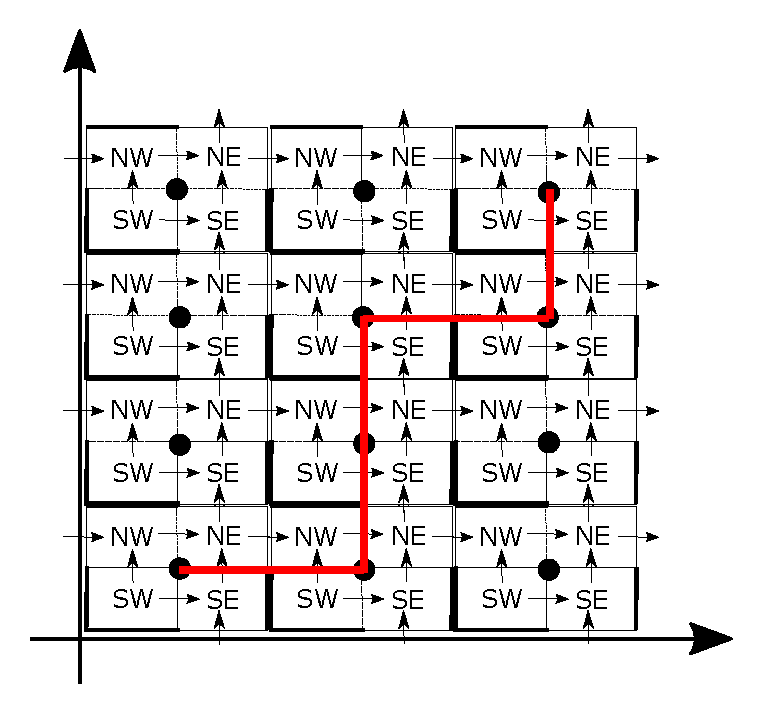
\includegraphics[width=0.55\columnwidth]{Image/ipp}
		\caption{\label{fig:ipp}IPP algoritmus}
	\end{figure}
\end{frame}

\begin{frame}{Initial-Route algoritmus}
\end{frame}

\begin{frame}{Detailed-Route algoritmus}
\end{frame}

\begin{frame}{Blocks}
  Three different block environments are pre-defined and may be styled with an
  optional background color.

  \begin{columns}[T,onlytextwidth]
    \column{0.5\textwidth}
      \begin{block}{Default}
        Block content.
      \end{block}

      \begin{alertblock}{Alert}
        Block content.
      \end{alertblock}

      \begin{exampleblock}{Example}
        Block content.
      \end{exampleblock}

    \column{0.5\textwidth}

      \metroset{block=fill}

      \begin{block}{Default}
        Block content.
      \end{block}

      \begin{alertblock}{Alert}
        Block content.
      \end{alertblock}

      \begin{exampleblock}{Example}
        Block content.
      \end{exampleblock}

  \end{columns}
\end{frame}

\section{Konklúzió}

\begin{frame}{Összefoglaló}
  Bemutattunk egy determinisztikus packet routing algoritmust, mely megoldott egy nyitott kérdést, de számos más kérdés még mindig nyitva hagyott. Például, hogy mi történik nem centralizált esetben?
  \begin{table}
  	\begin{tabular}{ c c c c c }
  		\toprule
  		Ref. & Dim. & Comp. Ratio & Determ? & $ B, c $ \\
  		\midrule
  			\cite{even2010logn, even2011online, evenM14} & 1 & $ O(log(n)) $ & Yes & $ B, c > log n, B/c = n^{O(1)} $ \\
  			\cite{angelov2009network} & 1 & $ O(log^3(n)) $ & No & $ B \geq 2, c = 1 $ \\
			\cite{azar2005packet} & 1 & $ O(log^2(n)) $ & No & $ B \geq 2, c = 1 $ \\
			\cite{even2010logn, evenM14} & 1 & $ O(log(n)) $ & No & $ B \in [1, log n], c \geq 1 $ \\
			\cite{even2011online, evenM14} & 1 & $ O(log^5(n)) $ & Yes & $ [3, O(log n)] $ \\
			\cite{even2011online, evenM14} & d & $ O(log^{d+4}(n)) $ & Yes & $ [5, O(log n)] $ \\
			\hline
			\cite{even2015better} & 1 & $ O(log(n)) $ & Yes & $ [5, O(log n)] $ \\
		\bottomrule
	\end{tabular}
	\caption{Összehasonlítás más algoritmusokkal}
  \end{table}
\end{frame}

\appendix

\begin{frame}[allowframebreaks]{References}
	
	\bibliography{demo}
	\bibliographystyle{unsrt}
	
\end{frame}

\begin{frame}[standout]
  Kérdések?
\end{frame}

\begin{frame}[standout]
	Köszönjük a figyelmet!
\end{frame}

\end{document}
